\chapter{Learning Rappresentation}
\section{Introduzione}
Uno degli obiettivi fondamentali del Deep Learning è imparare rappresentazioni significative a partire da dei dati grezzi. Un buon modello di Deep Learning non si limita a classificare gli input, ma è in grado di riuscire a estrarre delle caratteristiche gerarchiche le quali semplificano notevolmente i compiti di analisi e previsione.

\section{Classificatori Lineari e i loro Limiti}
I classificatori lineari, i quali solitamente ci siamo trovati durante il corso di Machine Learning a interfacciarci, suddividono lo spazio degli input in due regioni separate da un iperpiano. Tuttavia, questa soluzione risulta essere molto limitata:
\begin{itemize}
    \item Non è in grado di gestire problemi con dati non linearmente separabili;
    \item La probabilità che una distribuzione casuale di punti $P$ sia separabile linearmente diminuisce all'aumentare della dimensionalità $N$ nel momento in cui $P \ge N$ (Teorema di Cover, 1966).
\end{itemize}

Per forza di cose nel caso in cui andassimo ad aumentare la dimensione di $N$ per cercare di arginare il problema, a causa del teorema di Cover dobbiamo fare anche attenzione anche alla \textit{Curse of Dimensionality}, la quale è anch'essa campo di studio.

\begin{figure}[!ht]
    \centering
    \begin{subfigure}[b]{0.45\textwidth}
        \centering
        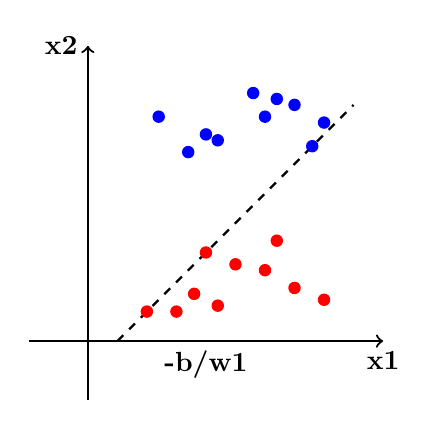
\begin{tikzpicture}[scale=0.75]
            \draw[->, thick] (-1,0) -- (5,0) node[anchor=north] {\textbf{x1}};
            \draw[->, thick] (0,-1) -- (0,5) node[anchor=east] {\textbf{x2}};
            \node[below] at (2,0) {\textbf{-b/w1}};
            \draw[thick, dashed] (0.5,0) -- (4.5,4);
            \foreach \x/\y in {
                2/3.5, 1.2/3.8, 3.5/4, 2.8/4.2, 4/3.7,
                3.8/3.3, 3.2/4.1, 2.2/3.4, 3/3.8, 1.7/3.2
            } {
                \fill[blue] (\x,\y) circle (3pt);
            }
            \foreach \x/\y in {
                1/0.5, 2/1.5, 1.8/0.8, 3/1.2, 4/0.7,
                2.5/1.3, 3.5/0.9, 1.5/0.5, 3.2/1.7, 2.2/0.6
            } {
                \fill[red] (\x,\y) circle (3pt);
            }
        \end{tikzpicture}
        \caption{Dati linearmente separabili}
    \end{subfigure}
    \hfill
    \begin{subfigure}[b]{0.45\textwidth}
        \centering
        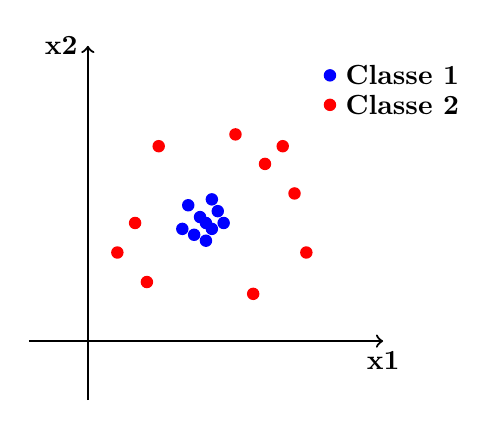
\begin{tikzpicture}[scale=0.75]
            \draw[->, thick] (-1,0) -- (5,0) node[anchor=north] {\textbf{x1}};
            \draw[->, thick] (0,-1) -- (0,5) node[anchor=east] {\textbf{x2}};
            \foreach \x/\y in {
                2/2, 2.2/2.2, 1.8/1.8, 2.1/1.9, 1.9/2.1,
                2/1.7, 2.3/2, 1.7/2.3, 2.1/2.4, 1.6/1.9
            } {
                \fill[blue] (\x,\y) circle (3pt);
            }
            \foreach \x/\y in {
                1/1, 3/3, 3.5/2.5, 2.5/3.5, 1.2/3.3,
                3.7/1.5, 0.8/2, 3.3/3.3, 2.8/0.8, 0.5/1.5
            } {
                \fill[red] (\x,\y) circle (3pt);
            }
            \fill[blue] (4.1,4.5) circle (3pt);
            \node[right] at (4.2,4.5) {\textbf{Classe 1}};
            \fill[red] (4.1,4) circle (3pt);
            \node[right] at (4.2,4) {\textbf{Classe 2}};
        \end{tikzpicture}
        \caption{Dati non linearmente separabili}
    \end{subfigure}

    \caption{Confronto tra un dataset linearmente separabile (a sinistra) e uno non linearmente separabile (a destra).}
    \label{fig:linear-vs-non-linear}
\end{figure}

\subsection{Soluzione: Rappresentazioni (Features)}
Per superare i limiti dei classificatori lineari, ci sono varie metodologie, una di queste è quella approfondita attraverso l'esempio della funzione \textbf{XOR}, visto nel corso di Machine Learning, dove per definizione la funzione XOR genera dei dati che non sono linearmente separabili, ma attraverso la combinazione di modelli più semplici, i quali ci permettono di attura la separabilità lineare, riusciamo a ottenere la funzione complessiva attraverso una rete neurale. Di seguito alcune metodologie per far fronte ai limiti dei classificatori lineari:
\begin{itemize}
    \item Estrarre caratteristiche rilevanti dall'input grezzo;
    \item Trasformare i dati in una rappresentazione in cui la separabilità lineare sia più semplice;
    \item Usare estrattori di caratteristiche non lineari, come reti neurali profonde.
\end{itemize}

\section{Metodi di Estrazione}
Alcuni metodi per estrarre caratteristiche utili includono:
\begin{itemize}
    \item \textbf{Tiling dello spazio}: suddivisione dello spazio in regioni più piccole.
    \item \textbf{Proiezioni casuali}: trasformazioni casuali per aumentare la dimensione dello spazio.
    \item \textbf{Classificatori polinomiali}: utilizzo di combinazioni di variabili di input per migliorare la separabilità.
    \item \textbf{Macchine a kernel}: mappatura non lineare dei dati in uno spazio a più alta dimensionalità.
\end{itemize}

Generalmente l'idea alla base di tutte queste possibilità è quella di poter espandere le dimensioni della nostra rappresentazione, per far sì che i nostri dati risultino essere facilmente lineramente separabili.

\begin{Osservazione}
    Ci potremmo chiedere del perché dovremmo usare soltanto le features in maniera lineare. La risposte è che diventa più semplice nella pratica, poiché nel momento in cui vado a considerare delle features che non lo sono, tutto risulterà più complesso a livello di costo computazionale.
\end{Osservazione}

\section{Reti Neurali Poco Profonde}
Per poter far fronte a quesat problemati, si possono utilizzare le strategie quì di seguito elencate:

\begin{itemize}
    \item Le macchine a vettori di supporto (SVM) e i metodi a kernel utilizzano uno strato con funzioni di base non lineari, seguito da uno strato lineare;
    \item Utilizzare delle reti neurali con due strati diventando degli approssimatori universali~\ref{th:Cybenko_1989}, tuttavia richiedono un numero elevato di neuroni per rappresentare funzioni complesse.
\end{itemize}

\begin{Teorema}
    Una rete con 2 strati (con 1 strato nascosto), è un approssimatore universale, può cioè approssimare in modo arbitrariamente preciso ogni funzione continua $g(u_1,u_2,\dots,u_d)$ (pur di prendere un numero sufficiente di neuroni).
    \label{th:Cybenko_1989}
\end{Teorema}

A fronte di questo teorema potremmo chiederci del perché con il Deep Learning, ci dobbiamo spingere a utilizzare delle reti neurali più profonde, visto che ogni funzione continua sia possibile rappresentarla anche con semplicemente un singolo layer nascosto.

\subsubsection{Perché le Architetture Profonde?}
La risposta viene trovata facilmente, poiché una rete neurale profonda è in grado di rappresentare funzioni complesse in modo più efficiente rispetto a una rete poco profonda, ma soprattuto, nel momento in cui passiamo a una rete neurale più profonda avremo un risultato in meno tempo, quindi abbiamo rinunciato a dello spazio per risparmiare del tempo. Inoltre esse hanno:
\begin{itemize}
    \item Maggiore capacità di modellare strutture gerarchiche nei dati  (es. riconoscimento visivo, riconosco una figura a seconda di sue diverse caratteristiche, ognuna analizzata in un layer);
    \item Possibilità di apprendere trasformazioni sempre più astratte dei nostri dati.
\end{itemize}

\section{Ipotesi del Manifold}
Un concetto molto importante del Deep Learning è l'ipotesi del \textbf{Manifold}, se volessimo riconoscere la faccia di una persona prendendo in analisi quella nella Figura~\ref{fig:manifold}, noi possiamo notare che in ognuna delle sottofigure vi è la stessa persona, è corretto interrogarsi sul perché noi umani, riusciamo a dire ciò. Molto semplicemente ci sono delle caratteristiche che noi riusciamo a riconoscere che appartengono alla stessa persona. Il nostro cervello, e più in generale, la nostra realtà si trova in uno spazio dimensionale che non è della stessa grandezza della figura che possiamo creare.

\begin{figure}[h]
    \centering
    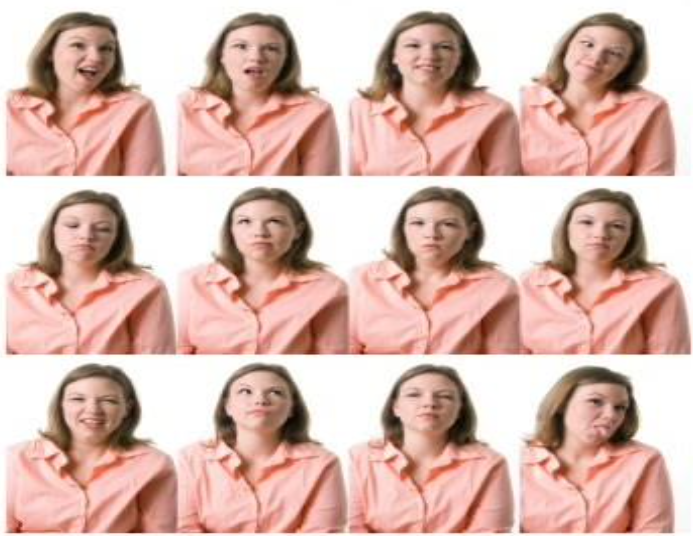
\includegraphics[width=0.45\textwidth]{figure/Manifold.png}
    \caption{Esempio dell'ipotesi del manifold.}
    \label{fig:manifold}
\end{figure}

\marginpar{L'argomento della Data Manifold, viene trattato di più in: \href{https://ieeexplore.ieee.org/stamp/stamp.jsp?tp=&arnumber=1640964}{Hadsell et al. CVPR 2006~\cite{hadsell2006dimensionality}}}

È stato dimostrato come noi umani, siamo in grado di riconoscere una faccia di una persona rappresentando meno di 56 variabili, mentre differentemente nel momento in cui usiamo un'immagine composta da $1000$x$1000$ pixel avrò $1\,000\,000$ di dimensioni per il nostro calcolatore. Questa è la così detta ipotesi del Manifold, ossia che la realtà vive in una dimensione molto minore rispetto alla dimensione che utiliziamo per rappresentarla. 

\subsubsection{Correlazione con cio che stiamo facendo}
Se avessimo un estrattore ideale, potremmo essere in grado di prendere questa immagine da un milione di dimensioni, e semplicemente estrarre queste 56 features, in modo tale da essere in grado di riconoscere l'immagine. Pertanto noteremo come muovendoci su un piano cartesiano, spostandoci lungo una singola dimensione cambieremo solo ed esclusivamente una singola features (Figura~\ref{fig:cartesianFig}).

\begin{figure}
    \centering
    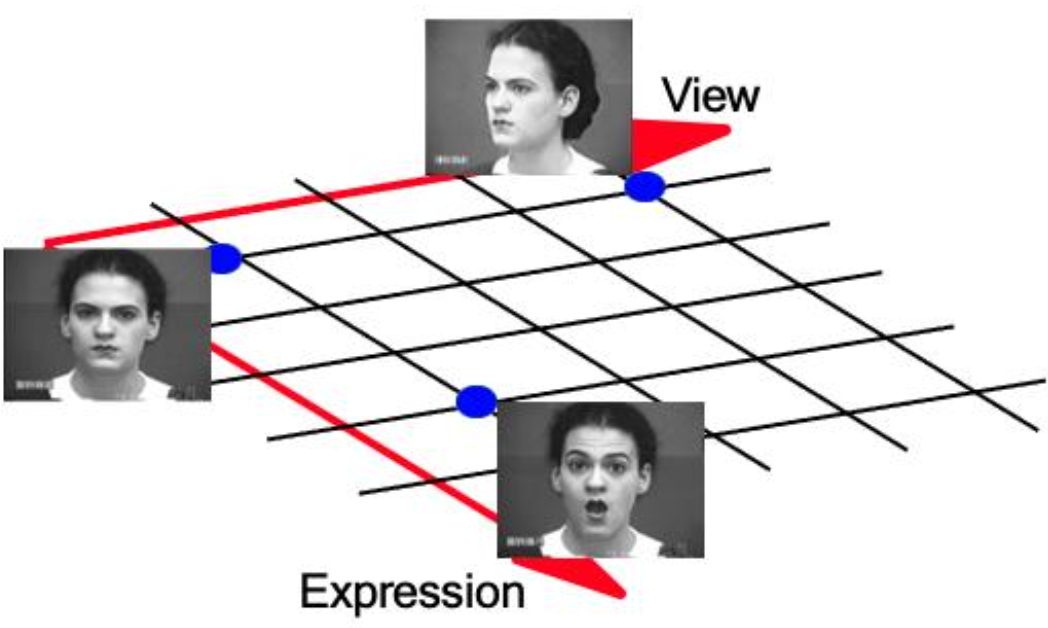
\includegraphics[width=0.45\linewidth]{figure/cartesianFig.png}
    \caption{Rappresentazione di una possibile idealizzazione su un piano cartesiano di un estrattore di features}
    \label{fig:cartesianFig}
\end{figure}
\section{Struttura Gerarchica dei Dati}
Le architetture multilivello riflettono la natura composizionale dei dati, analizzando le parti di esse di volta in volta, queste possono diventare delle ottime possibilità per spostarci verso un estrattore ideale, permettendo un'efficiente rappresentazione delle informazioni:

\begin{itemize}
    \item \textbf{Visione}: pixel $\Rightarrow$ bordi $\Rightarrow$ texture $\Rightarrow$ oggetti
    \item \textbf{Testo}: caratteri $\Rightarrow$ parole $\Rightarrow$ frasi $\Rightarrow$ discorso
    \item \textbf{Audio}: campioni $\Rightarrow$ bande spettrali $\Rightarrow$ fonemi $\Rightarrow$ parole
\end{itemize}

\section{Conclusione}
Le reti neurali profonde pertanto non fanno altro che bilanciare tempo e spazio, facendo sì che più livelli implicano più operazioni sequenziali, riducono la necessità di risorse computazionali parallele e infine consentono una rappresentazione più compatta delle funzioni complesse.